\documentclass[twoside,a4paper]{article}
\usepackage{geometry}
\geometry{margin=1.5cm, vmargin={0pt,1cm}}
\setlength{\topmargin}{-1cm}
\setlength{\paperheight}{29.7cm}
\setlength{\textheight}{25.3cm}

% useful packages.
\usepackage{amsfonts}
\usepackage{amsmath}
\usepackage{amssymb}
\usepackage{amsthm}
\usepackage{enumerate}
\usepackage{graphicx}
\usepackage{multicol}
\usepackage{fancyhdr}
\usepackage{layout}

% some common command
\newcommand{\dif}{\mathrm{d}}
\newcommand{\avg}[1]{\left\langle #1 \right\rangle}
\newcommand{\difFrac}[2]{\frac{\dif #1}{\dif #2}}
\newcommand{\pdfFrac}[2]{\frac{\partial #1}{\partial #2}}
\newcommand{\OFL}{\mathrm{OFL}}
\newcommand{\UFL}{\mathrm{UFL}}
\newcommand{\fl}{\mathrm{fl}}
\newcommand{\op}{\odot}
\newcommand{\Eabs}{E_{\mathrm{abs}}}
\newcommand{\Erel}{E_{\mathrm{rel}}}

\begin{document}

\pagestyle{fancy}
\fancyhead{}
\lhead{NAME Jiatu Yan}
\chead{Numerical Analysis homework \#7}
\rhead{Date 2020.5.24}


\section*{I. \small{Can we compute the root with absolute accuracy $<10^{-6}$ ?}}
We start the bisection method with the interval $[128,129]$, and the interval will be shorten by half after one iteration.
Assume that the interval after the n-th iteration is $[a_n,b_n]$,  $a_0=128=1\times2^{7}$ $b_0=129=\left( 1+2^{-7} \right)\times2^{7} $, $n\le$ the iteration times.
We can easily find that $a_n\in\mathcal{F}$,  $b_n\in\mathcal{F}$ until $a_n$'s or $b_n$'s mantissa contains $2^{-23}$ and the iteration will end.
So we know the iteration will end when $b_n-a_n=2^{23}\times2^{7}=\epsilon_M\times2^{7}$.  

Thus we have $\max E_abs=\epsilon_u\times2^{7}=2^{-17}\thickapprox 7.629\times_{10}^{-6}>10^{-6}$.
So the absolute accuracy may be bigger than $10^{-6}$.

\section*{II. \small{What are the condition numbers of the following functions?Where are they large?}}

\subsection*{II-a \small{$\left( x-1 \right)^{\alpha} $.}}
\[
	C_f\left( x \right)= \mid \frac{x\alpha\left( x-1 \right)^{\alpha-1} }{\left( x-1 \right)^{\alpha} } \mid
	= \mid \frac{\alpha x}{x-1} \mid 
	\to \infty \quad \mathrm{when} \quad x\to 1
.\] 
\subsection*{II-b \small{$\ln x$.}}
\[
	C_f\left( x \right) = \mid \frac{x \frac{1}{x}}{\ln x} \mid = \mid \frac{1}{\ln x} \mid 
	\to \infty \quad \mathrm{when} \quad x\to 1
.\] 

\subsection*{II-c \small{$e^{x}$.}}
\[
	C_f\left( x \right) = \mid \frac{xe^{x}}{e^{x}} \mid = \mid x \mid
.\] 

The $C_f\left( x \right) $ will be large when $x$ is large.
\subsection*{II-d \small{$\arccos x$.}}
\[
	C_f\left( x \right)= \mid \frac{x \frac{-1}{\sqrt{1-x^{2}} }}{\arccos x} \mid = \mid \frac{x}{\arccos x \sqrt{1-x^{2}} } \mid 
.\] 

Since $\sqrt{1-x^{2}}=o\left( x \right)  $ and $\arccos x$ is bouded, we have $C_f\left( x \right) \to\infty 
\quad \mathrm{when} \quad x\to \pm 1\quad$.   
\section*{III. \small{The last Exercise in Section 1.3.5 in the notes.}}
\begin{equation*}
	\begin{split}
		\mathrm{cond}_f\left( x \right)&= \mid \frac{xf'\left( x \right) }{f\left( x \right) } \mid 
		= \frac{x}{\sin x}\\
		f_A\left( x \right)&=\frac{\sin x\left( 1+\delta_2 \right) }
		{[1+\cos x\left( 1+\delta_1 \right) ]\left( 1+\delta_3 \right) }\left( 1+\delta_4 \right) 
		\qquad  \mid \delta_i \mid <\epsilon_u \\
				   &=\frac{\sin x}{1+\cos x}\left( 1-\frac{\cos x\delta_1}{1+\cos x+\cos x\delta_1} \right)
				   \frac{\left( 1+\delta_2 \right)\left( 1+\delta_4 \right)  }{\left( 1+\delta_3 \right) }\\
				   &\thickapprox \frac{\sin x}{1+ \cos x}
				   \left( 1+\delta_2+\delta_4-\delta_3-\frac{\cos x}{1+\cos x}\delta_1 \right)\\
		\Longrightarrow&\varphi\left( x \right) =3+\frac{\cos x}{1+\cos x}\\
		\therefore \mathrm{cond}_A\left( x \right)&\le \frac{\sin x}{x}\left( 3+\frac{\cos x}{1+\cos x} \right).  
	\end{split}	
\end{equation*}
\section*{IV. \small{Consider the function $f\left( x \right)=1-e^{-x}$ for $x\in[0,1]$.}}
\subsection*{IV-a \small{Show that cond$_f\left( x \right)\le 1 $ for $x\in[0,1]$.}}
\[
	\mathrm{cond}_f\left( x \right)= \mid \frac{-xe^{-x}}{1-e^{-x}} \mid =\frac{x}{e^{x} - 1} 
.\] 
Because $e^{x}-1=o\left( x \right)\quad \mathrm{when}\quad x\to 0$
, so $\mathrm{cond}_f\left( x \right)\to1\quad \mathrm{when}\quad x\to 0 $. 

Assume $g_1\left( x \right) =x$, $g_2\left( x \right)=e^{x}-1 $. 
Because $g_1\left( 0 \right)=g_2\left( 0 \right)= 0 $, $\forall x\in[0,1]\quad g'_1\left( x \right)=1\le e^{x}=g'_2\left( x \right)$
, we have $\forall x\in[0,1]\quad g_1\left( x \right)\le g_2\left( x \right)  $. 
Thus $\mathrm{cond}_f\left( x \right)\le 1 $. 

\subsection*{IV-b \small{Estimate cond$_A\left( x \right) $ for $x\in[0,1]$.}}
\begin{equation*}
	\begin{split}
		A&=\left( 1-e^{-x}\left( 1+ \delta_1\right)  \right) \left( 1+\delta_2 \right) \qquad \mid \delta_i \mid<\epsilon_u\\
		 &=\left( 1-e^{-x} \right)\left( 1+\delta_2-\frac{1}{e^{x}-1}\delta_1\left( \delta_2+1 \right)  \right)\\
		 &\thickapprox\left( 1-e^{-x} \right)\left( 1+\delta_2-\frac{1}{e^{x}-1}\delta_1 \right)\\
		\Longrightarrow&\varphi\left( x \right) =  1+ \mid \frac{1}{e^{x}-1} \mid=\frac{e^{x}}{e^{x}-1}\\
		\therefore  \mathrm{cond}_A\left( x \right)&\le \frac{\varphi\left( x \right) }{\mathrm{cond}_f\left( x \right) }
		=\frac{e^{x}}{x}\to \infty\quad \mathrm{when}\quad x\to 0.
	\end{split}	
\end{equation*}
\subsection*{IV-c \small{Use c++ to plot $\mathrm{cond}_f\left( x \right) $ and $\mathrm{cond}_A\left( x \right) $ as a function of x on $[0,1]$.}}

\begin{figure}[ht]
        \centering
        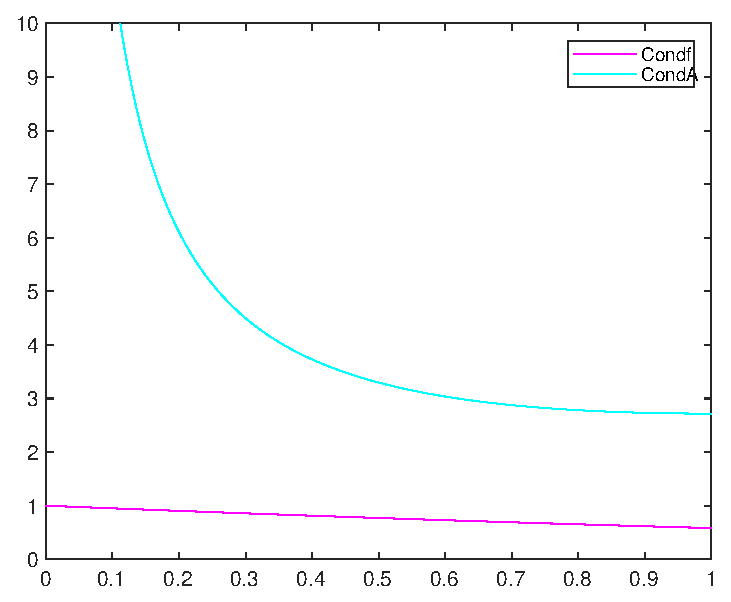
\includegraphics[width=15cm, height=8cm]{./Plot/result.eps}
	\caption{$\mathrm{cond}_f\left( x \right)$ and $\mathrm{cond}_A\left( x \right) $.}
\end{figure}

We find that $\mathrm{cond}_A\left( x \right) $ is far larger than 
$\mathrm{cond}_f\left( x \right) $ especially when x is close to zero.
$\mathrm{cond}_A\left( x \right) \to \infty$ when $x\to 0$, which satisfies the 
theorem that the subtraction in $1-e^{-x}$ is not accurate
, especially when $x\to 0$, $1-e^{-x}\to 0$.

\section*{V. \small{Derive the componentwise condition number of $f$ based on the 1-norm. And compare the result with that in the Wilkinson Example.}}
$r=f\left( a_0,a_1,\ldots,a_{n-1} \right) $, assume that $A=\left( a_0,a_1,\ldots,a_{n-1} \right) $.

We have $B=\left( b_j \right) $, where $b_j= \mid \frac{a_j\frac{\partial f}{\partial a_j}}{f\left( A \right) } \mid$, $j=0,1\ldots\left( n-1 \right) $.

As $f$ finds the root of polynomial $q\left( x\right)=0 $, the $\frac{\partial f}{\partial a_j}$ can be view as the change of the root when slightly change $a_j$. So we assume  $g\left( x \right)=x^{j} $, the new function is $F=q+\epsilon g$ and the root of  $F$ is  $r+h$, by corollary 1.43  $h\thickapprox -\epsilon \frac{g\left( r \right) }{q'\left( r \right) }$.So we have

\[
	\frac{\partial f}{\partial a_j}=\lim_{\epsilon\to 0}\frac{r-r+h}{\epsilon}\thickapprox -\frac{g\left( r \right) }{q'\left( r \right) }
	=-\frac{r^{j}}{\sum_{i=0}^{n-1}\left( i+1 \right)a_{i+1}r^{i} }
.\] 

So the componentwise condition number of $f\left( x \right) $ is 
\[
	\mathrm{cond}_f\left( x \right)= \mid  \mid B \mid  \mid _1=\sum_{j=0}^{n-1} 
	\frac{ \mid a_j \mid r^{j}}{ \mid q'\left( r \right)  \mid }
	=\sum_{j=0}^{n-1}\frac{\mid a_j \mid r^{j}}{\sum_{i=0}^{n-1}\left( i+1 \right)a_{i+1}r^{i}}
.\] 

In the Wilkinson Example, $q\left( x \right)=\prod_{k=1}^{p}\left( x-k \right)=\sum_{i=0}^{p}a_ix^{i}  $, so
\[
	\mathrm{cond}_f\left( x \right) =  \frac{\sum_{j=0}^{p-1} \mid a_j \mid p^{j}}{\left( p-1 \right)! } 
.\] 

Because $x^{p}=-\sum_{i=0}^{p-1}a_ix^{i}$, so
\[
	\frac{p^{p}}{\left( p-1 \right)! }=\frac{-\sum_{i=0}^{p-1}a_ip^{i}}{\left( p-1 \right)! }\le \mathrm{cond}_f\left( x \right) 
.\] 

Because in the Wilkinson Example, we calculate the change in the root for a small change in the highest item $x^{p}$. 
The change equals to that fix $a_p$ and slightly change  $a_i\quad\left( i=0,1\ldots,p-1 \right) $ uniformly.
While the componentwise condition number of f means the change in the root for small changes in the coefficient of 
$q\left( x \right) $, where $a_i\quad\left( i=0,1,\ldots,p-1 \right) $ can be changed seperately. So obviously the change in the latter
one includes the change in the formal one. So the result in the Wilkinson Example in the notes is smaller than the condition number
which we calculated in the problem.
\end{document}

%%% Local Variables: 
%%% mode: latex
%%% TeX-master: t
%%% End: 
